\documentclass{beamer}
\usepackage[english]{babel}
%\usepackage[utf8]{inputenc}
\usepackage[T1]{fontenc}
\usepackage{stmaryrd} %http://www.ctan.org/pkg/stmaryrd
\usepackage{amsmath} %http://www.ctan.org/pkg/amsmath
\usepackage{amssymb}
\usepackage{subfig}
\usepackage{hyperref}
\usepackage{tikz}
\usepgflibrary{decorations.pathreplacing}


\usetheme[usetitleprogressbar, numbering=fraction]{metropolis}

\graphicspath{{img/}}

\newcommand\bb{Benjamin Boisson}
\newcommand\gc{Guillaume Combette}
\newcommand\dl{Dimitri Lajou}
\newcommand\vl{Victor Lutfalla}
\newcommand\om{Octave Mariotti}
\newcommand\mr{Raphaël Monat}
\newcommand\me{Etienne Moutot} % He is not the only one author o/ Just that \em is already taken
\newcommand\js{Johanna Seif}
\newcommand\ps{Pijus Simonaitis}

\definecolor{Cerulean}{HTML}{5974EF}



\title{Blend'it}
\subtitle{Integrated project}
\author{\bb\\ \gc\\ \dl\\ \vl\\ \om\\ \mr\\ \me\\ \js\\ \ps\\}
\date{April 15th, 2016}

\begin{document}
\begin{frame}
\begin{figure}
  \begin{center}
    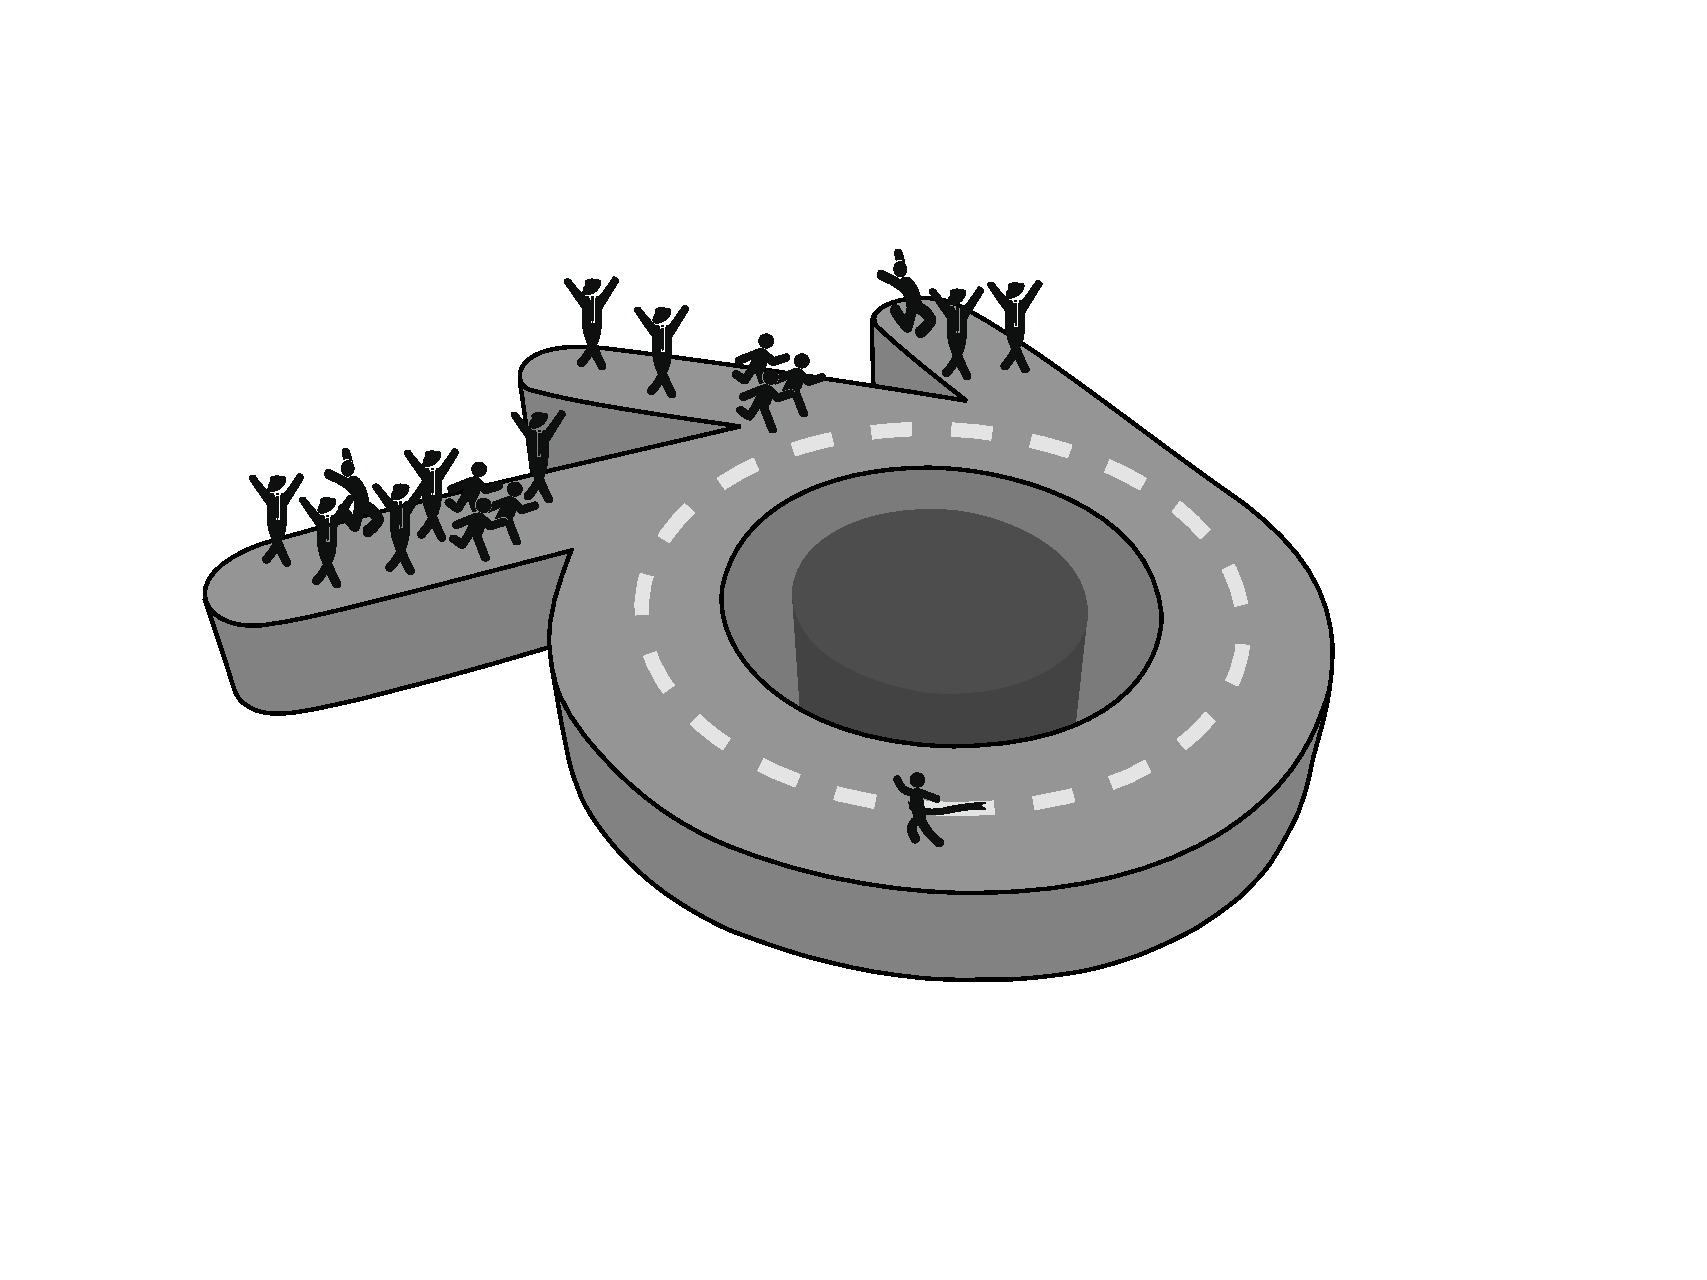
\includegraphics[width=8cm]{logo.pdf}
  \end{center}
\end{figure}
\end{frame}

\maketitle

\begin{frame}{Outline}
  \setbeamertemplate{section in toc}[sections numbered]
  \tableofcontents[hideallsubsections]
\end{frame}

\bgroup
\setbeamercolor{background canvas}{bg=black}
\begin{frame}[plain]{}
\end{frame}
\egroup

\section{What is Blend'it ?}
\begin{frame}{What is Blend'it ?}
  Blend'it is a \textbf{Blender plug-in} for \textbf{crowd animation} and \textbf{environment generation}.
  
  + screenshot
\end{frame}

\begin{frame}{A Lot of Powerful Software}


\begin{figure}
  \includegraphics<1>[width=.95\textwidth]{golaem.jpg}
  \includegraphics<2>[width=.95\textwidth]{massive.jpg}
  \includegraphics<3>[width=.95\textwidth]{VUE.jpg}
  \caption*{\only<1>{Golaem}\only<2>{Massive}\only<3>{VUE}}
\end{figure}

\end{frame}

\begin{frame}{A Lot of Expensive Software}
  \begin{itemize}
    \item Maya3D: \$1470/year
    \item Golaem: \$5000/year
    \item Massive: \$3,500 - \$16,000/year
    \item VUE: \$1700
    \item Terragen: \$600
  \end{itemize}
\end{frame}

\begin{frame}{Why Blender ?}
  Complete open-source 3D software: modelisation, animation, render, ...
    \begin{figure}
        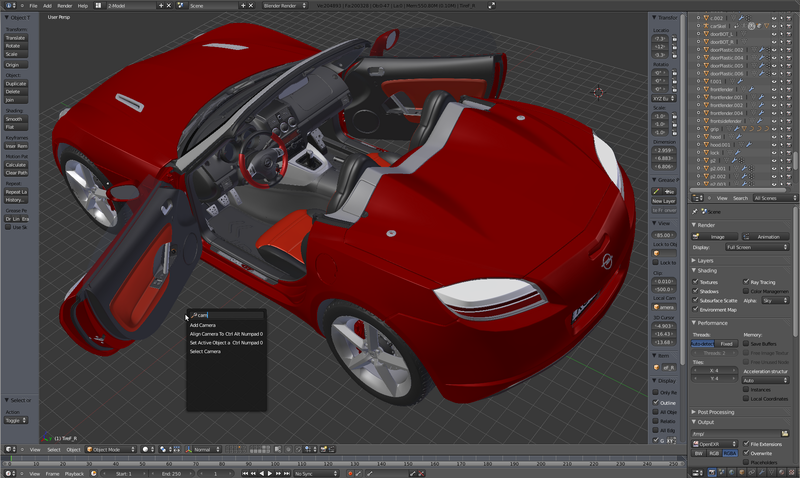
\includegraphics[width=10cm]{blender_mod}
    \end{figure}
\end{frame}

\begin{frame}{Why Blender ?}
  Powerful python API (no need to modify the source code of blender)
  \begin{figure}
        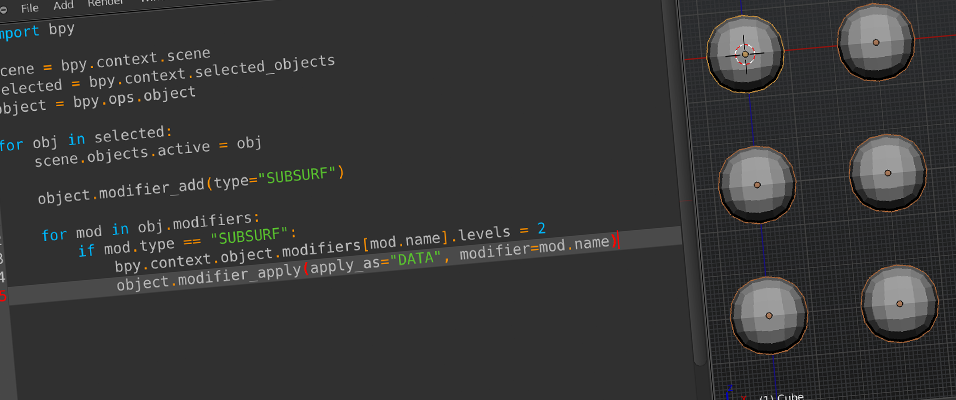
\includegraphics[width=11cm]{blender_script}
    \end{figure}
\end{frame}

\begin{frame}{Project organization}
  \begin{figure}
    \begin{center}
      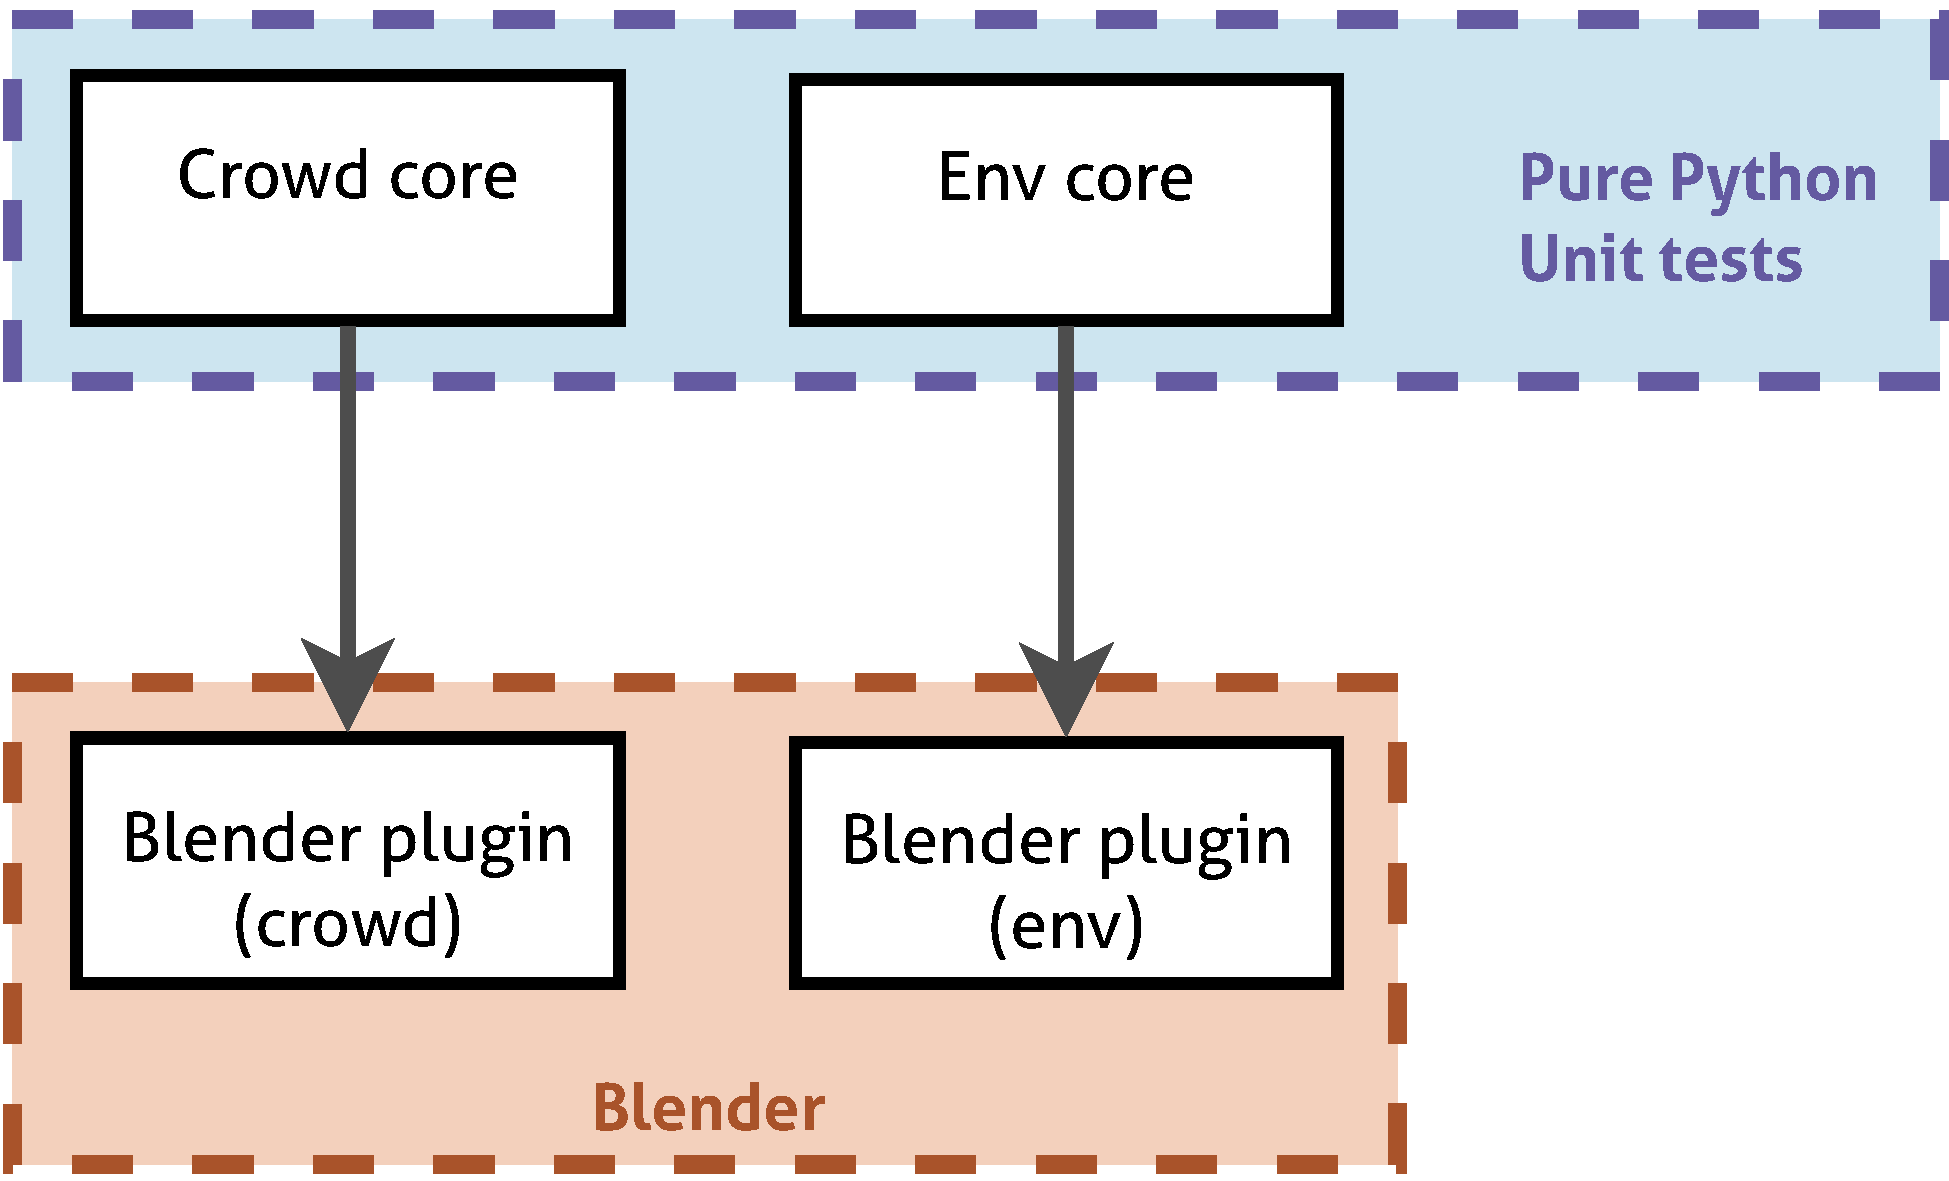
\includegraphics[width=9cm]{orga.pdf}
    \end{center}
  \end{figure}
\end{frame}


\section{Crowd Animation}
\begin{frame}{Crowd Animation - Algorithm}
\begin{itemize}
  \item Goal: animation of moving crowds.
  \item Two issues: \textbf{path generation}, individual movements.
  % Talk about the fact that after a few of researches, individual movements appeared to be much more difficult that we thought: problem of coordination of foots, arms...
  % That is why all we will talk about is the generation of the path
  \item Strategy: least-effort path.
  % TODO tiks drawing to explain the shortest path
  % We assume that our individuals have an objective and the trajectory is optimised by computing the minimum energy cost between the starting point and the objective.
  % TODO graph that explains the algorithm to be able to explain it on the drawing. Talk about how we make the graph: one node per individual and grid pattern
  % Computation of the shortest path thanks to A* algorithm
  % We decided not to use the graph because of computation time 
\end{itemize}

\begin{figure}[h!]
  \centering
  \scalebox{.4}{% Graphic for TeX using PGF
% Title: /home/johanna/Documents/Informatique/M1/Projet/pib/beamer_final/short_path.dia
% Creator: Dia v0.97.3
% CreationDate: Wed Apr 13 17:17:40 2016
% For: johanna
% \usepackage{tikz}
% The following commands are not supported in PSTricks at present
% We define them conditionally, so when they are implemented,
% this pgf file will use them.
\ifx\du\undefined
  \newlength{\du}
\fi
\setlength{\du}{15\unitlength}
\begin{tikzpicture}
\pgftransformxscale{1.000000}
\pgftransformyscale{-1.000000}
\definecolor{dialinecolor}{rgb}{0.000000, 0.000000, 0.000000}
\pgfsetstrokecolor{dialinecolor}
\definecolor{dialinecolor}{rgb}{1.000000, 1.000000, 1.000000}
\pgfsetfillcolor{dialinecolor}
\pgfsetlinewidth{0.200000\du}
\pgfsetdash{}{0pt}
\pgfsetdash{}{0pt}
\pgfsetbuttcap
{
\definecolor{dialinecolor}{rgb}{0.000000, 0.000000, 0.000000}
\pgfsetfillcolor{dialinecolor}
% was here!!!
\definecolor{dialinecolor}{rgb}{0.000000, 0.000000, 0.000000}
\pgfsetstrokecolor{dialinecolor}
\draw (45.000000\du,-13.000000\du)--(75.000000\du,-10.000000\du);
}
\pgfsetlinewidth{0.200000\du}
\pgfsetdash{}{0pt}
\pgfsetdash{}{0pt}
\pgfsetmiterjoin
\pgfsetbuttcap
{
\definecolor{dialinecolor}{rgb}{0.000000, 0.000000, 0.000000}
\pgfsetfillcolor{dialinecolor}
% was here!!!
\definecolor{dialinecolor}{rgb}{0.000000, 0.000000, 0.000000}
\pgfsetstrokecolor{dialinecolor}
\pgfpathmoveto{\pgfpoint{75.000000\du}{-10.000000\du}}
\pgfpathcurveto{\pgfpoint{77.000000\du}{-4.000000\du}}{\pgfpoint{77.000000\du}{6.000000\du}}{\pgfpoint{77.000000\du}{6.000000\du}}
\pgfusepath{stroke}
}
\pgfsetlinewidth{0.200000\du}
\pgfsetdash{}{0pt}
\pgfsetdash{}{0pt}
\pgfsetbuttcap
{
\definecolor{dialinecolor}{rgb}{0.000000, 0.000000, 0.000000}
\pgfsetfillcolor{dialinecolor}
% was here!!!
\definecolor{dialinecolor}{rgb}{0.000000, 0.000000, 0.000000}
\pgfsetstrokecolor{dialinecolor}
\draw (50.000000\du,-7.000000\du)--(70.000000\du,-5.000000\du);
}
\pgfsetlinewidth{0.200000\du}
\pgfsetdash{}{0pt}
\pgfsetdash{}{0pt}
\pgfsetbuttcap
{
\definecolor{dialinecolor}{rgb}{0.000000, 0.000000, 0.000000}
\pgfsetfillcolor{dialinecolor}
% was here!!!
\definecolor{dialinecolor}{rgb}{0.000000, 0.000000, 0.000000}
\pgfsetstrokecolor{dialinecolor}
\draw (70.000000\du,-5.000000\du)--(70.000000\du,2.000000\du);
}
\pgfsetlinewidth{0.200000\du}
\pgfsetdash{}{0pt}
\pgfsetdash{}{0pt}
\pgfsetmiterjoin
\pgfsetbuttcap
{
\definecolor{dialinecolor}{rgb}{0.000000, 0.000000, 0.000000}
\pgfsetfillcolor{dialinecolor}
% was here!!!
\definecolor{dialinecolor}{rgb}{0.000000, 0.000000, 0.000000}
\pgfsetstrokecolor{dialinecolor}
\pgfpathmoveto{\pgfpoint{50.000000\du}{-7.000000\du}}
\pgfpathcurveto{\pgfpoint{50.000000\du}{2.000000\du}}{\pgfpoint{67.676000\du}{2.000000\du}}{\pgfpoint{70.000000\du}{2.000000\du}}
\pgfusepath{stroke}
}
\pgfsetlinewidth{0.200000\du}
\pgfsetdash{}{0pt}
\pgfsetdash{}{0pt}
\pgfsetbuttcap
\pgfsetmiterjoin
\pgfsetlinewidth{0.200000\du}
\pgfsetbuttcap
\pgfsetmiterjoin
\pgfsetdash{}{0pt}
\definecolor{dialinecolor}{rgb}{1.000000, 1.000000, 1.000000}
\pgfsetfillcolor{dialinecolor}
\fill (72.000000\du,-7.000000\du)--(72.750000\du,-7.250000\du)--(73.000000\du,-8.000000\du)--(73.250000\du,-7.250000\du)--(74.000000\du,-7.000000\du)--(73.250000\du,-6.750000\du)--(73.000000\du,-6.000000\du)--(72.750000\du,-6.750000\du)--cycle;
\definecolor{dialinecolor}{rgb}{0.000000, 0.000000, 0.000000}
\pgfsetstrokecolor{dialinecolor}
\draw (72.000000\du,-7.000000\du)--(72.750000\du,-7.250000\du)--(73.000000\du,-8.000000\du)--(73.250000\du,-7.250000\du)--(74.000000\du,-7.000000\du)--(73.250000\du,-6.750000\du)--(73.000000\du,-6.000000\du)--(72.750000\du,-6.750000\du)--cycle;
\pgfsetbuttcap
\pgfsetmiterjoin
\pgfsetdash{}{0pt}
\definecolor{dialinecolor}{rgb}{0.000000, 0.000000, 0.000000}
\pgfsetstrokecolor{dialinecolor}
\draw (72.000000\du,-7.000000\du)--(72.750000\du,-7.250000\du)--(73.000000\du,-8.000000\du)--(73.250000\du,-7.250000\du)--(74.000000\du,-7.000000\du)--(73.250000\du,-6.750000\du)--(73.000000\du,-6.000000\du)--(72.750000\du,-6.750000\du)--cycle;
\pgfsetlinewidth{0.200000\du}
\pgfsetdash{}{0pt}
\pgfsetdash{}{0pt}
\pgfsetbuttcap
\pgfsetmiterjoin
\pgfsetlinewidth{0.200000\du}
\pgfsetbuttcap
\pgfsetmiterjoin
\pgfsetdash{}{0pt}
\definecolor{dialinecolor}{rgb}{1.000000, 1.000000, 1.000000}
\pgfsetfillcolor{dialinecolor}
\fill (47.500000\du,-10.499997\du)--(48.000000\du,-9.499997\du)--(47.000000\du,-9.499997\du)--cycle;
\definecolor{dialinecolor}{rgb}{1.000000, 0.027451, 0.027451}
\pgfsetstrokecolor{dialinecolor}
\draw (47.500000\du,-10.499997\du)--(48.000000\du,-9.499997\du)--(47.000000\du,-9.499997\du)--cycle;
\pgfsetlinewidth{0.200000\du}
\pgfsetdash{}{0pt}
\pgfsetdash{}{0pt}
\pgfsetbuttcap
\pgfsetmiterjoin
\pgfsetlinewidth{0.200000\du}
\pgfsetbuttcap
\pgfsetmiterjoin
\pgfsetdash{}{0pt}
\definecolor{dialinecolor}{rgb}{1.000000, 1.000000, 1.000000}
\pgfsetfillcolor{dialinecolor}
\fill (56.500000\du,-8.000000\du)--(57.000000\du,-7.000000\du)--(56.000000\du,-7.000000\du)--cycle;
\definecolor{dialinecolor}{rgb}{0.000000, 0.000000, 0.000000}
\pgfsetstrokecolor{dialinecolor}
\draw (56.500000\du,-8.000000\du)--(57.000000\du,-7.000000\du)--(56.000000\du,-7.000000\du)--cycle;
\pgfsetlinewidth{0.200000\du}
\pgfsetdash{}{0pt}
\pgfsetdash{}{0pt}
\pgfsetbuttcap
\pgfsetmiterjoin
\pgfsetlinewidth{0.200000\du}
\pgfsetbuttcap
\pgfsetmiterjoin
\pgfsetdash{}{0pt}
\definecolor{dialinecolor}{rgb}{1.000000, 1.000000, 1.000000}
\pgfsetfillcolor{dialinecolor}
\fill (56.500000\du,-11.000000\du)--(57.000000\du,-10.000000\du)--(56.000000\du,-10.000000\du)--cycle;
\definecolor{dialinecolor}{rgb}{0.000000, 0.000000, 0.000000}
\pgfsetstrokecolor{dialinecolor}
\draw (56.500000\du,-11.000000\du)--(57.000000\du,-10.000000\du)--(56.000000\du,-10.000000\du)--cycle;
\pgfsetlinewidth{0.200000\du}
\pgfsetdash{}{0pt}
\pgfsetdash{}{0pt}
\pgfsetbuttcap
\pgfsetmiterjoin
\pgfsetlinewidth{0.200000\du}
\pgfsetbuttcap
\pgfsetmiterjoin
\pgfsetdash{}{0pt}
\definecolor{dialinecolor}{rgb}{1.000000, 1.000000, 1.000000}
\pgfsetfillcolor{dialinecolor}
\fill (59.500000\du,-11.000000\du)--(60.000000\du,-10.000000\du)--(59.000000\du,-10.000000\du)--cycle;
\definecolor{dialinecolor}{rgb}{0.000000, 0.000000, 0.000000}
\pgfsetstrokecolor{dialinecolor}
\draw (59.500000\du,-11.000000\du)--(60.000000\du,-10.000000\du)--(59.000000\du,-10.000000\du)--cycle;
\pgfsetlinewidth{0.200000\du}
\pgfsetdash{}{0pt}
\pgfsetdash{}{0pt}
\pgfsetbuttcap
\pgfsetmiterjoin
\pgfsetlinewidth{0.200000\du}
\pgfsetbuttcap
\pgfsetmiterjoin
\pgfsetdash{}{0pt}
\definecolor{dialinecolor}{rgb}{1.000000, 1.000000, 1.000000}
\pgfsetfillcolor{dialinecolor}
\fill (59.500000\du,-8.000000\du)--(60.000000\du,-7.000000\du)--(59.000000\du,-7.000000\du)--cycle;
\definecolor{dialinecolor}{rgb}{0.000000, 0.000000, 0.000000}
\pgfsetstrokecolor{dialinecolor}
\draw (59.500000\du,-8.000000\du)--(60.000000\du,-7.000000\du)--(59.000000\du,-7.000000\du)--cycle;
\pgfsetlinewidth{0.200000\du}
\pgfsetdash{}{0pt}
\pgfsetdash{}{0pt}
\pgfsetbuttcap
\pgfsetmiterjoin
\pgfsetlinewidth{0.200000\du}
\pgfsetbuttcap
\pgfsetmiterjoin
\pgfsetdash{}{0pt}
\definecolor{dialinecolor}{rgb}{1.000000, 1.000000, 1.000000}
\pgfsetfillcolor{dialinecolor}
\fill (62.500000\du,-10.000000\du)--(63.000000\du,-9.000000\du)--(62.000000\du,-9.000000\du)--cycle;
\definecolor{dialinecolor}{rgb}{0.000000, 0.000000, 0.000000}
\pgfsetstrokecolor{dialinecolor}
\draw (62.500000\du,-10.000000\du)--(63.000000\du,-9.000000\du)--(62.000000\du,-9.000000\du)--cycle;
\pgfsetlinewidth{0.200000\du}
\pgfsetdash{}{0pt}
\pgfsetdash{}{0pt}
\pgfsetbuttcap
\pgfsetmiterjoin
\pgfsetlinewidth{0.200000\du}
\pgfsetbuttcap
\pgfsetmiterjoin
\pgfsetdash{}{0pt}
\definecolor{dialinecolor}{rgb}{1.000000, 1.000000, 1.000000}
\pgfsetfillcolor{dialinecolor}
\fill (62.500000\du,-7.000000\du)--(63.000000\du,-6.000000\du)--(62.000000\du,-6.000000\du)--cycle;
\definecolor{dialinecolor}{rgb}{0.000000, 0.000000, 0.000000}
\pgfsetstrokecolor{dialinecolor}
\draw (62.500000\du,-7.000000\du)--(63.000000\du,-6.000000\du)--(62.000000\du,-6.000000\du)--cycle;
\pgfsetlinewidth{0.200000\du}
\pgfsetdash{}{0pt}
\pgfsetdash{}{0pt}
\pgfsetbuttcap
\pgfsetmiterjoin
\pgfsetlinewidth{0.200000\du}
\pgfsetbuttcap
\pgfsetmiterjoin
\pgfsetdash{}{0pt}
\definecolor{dialinecolor}{rgb}{1.000000, 1.000000, 1.000000}
\pgfsetfillcolor{dialinecolor}
\fill (65.500000\du,-10.000000\du)--(66.000000\du,-9.000000\du)--(65.000000\du,-9.000000\du)--cycle;
\definecolor{dialinecolor}{rgb}{0.000000, 0.000000, 0.000000}
\pgfsetstrokecolor{dialinecolor}
\draw (65.500000\du,-10.000000\du)--(66.000000\du,-9.000000\du)--(65.000000\du,-9.000000\du)--cycle;
\pgfsetlinewidth{0.200000\du}
\pgfsetdash{}{0pt}
\pgfsetdash{}{0pt}
\pgfsetbuttcap
\pgfsetmiterjoin
\pgfsetlinewidth{0.200000\du}
\pgfsetbuttcap
\pgfsetmiterjoin
\pgfsetdash{}{0pt}
\definecolor{dialinecolor}{rgb}{1.000000, 1.000000, 1.000000}
\pgfsetfillcolor{dialinecolor}
\fill (64.500000\du,-7.000000\du)--(65.000000\du,-6.000000\du)--(64.000000\du,-6.000000\du)--cycle;
\definecolor{dialinecolor}{rgb}{0.000000, 0.000000, 0.000000}
\pgfsetstrokecolor{dialinecolor}
\draw (64.500000\du,-7.000000\du)--(65.000000\du,-6.000000\du)--(64.000000\du,-6.000000\du)--cycle;
\pgfsetlinewidth{0.200000\du}
\pgfsetdash{}{0pt}
\pgfsetdash{}{0pt}
\pgfsetbuttcap
\pgfsetmiterjoin
\pgfsetlinewidth{0.200000\du}
\pgfsetbuttcap
\pgfsetmiterjoin
\pgfsetdash{}{0pt}
\definecolor{dialinecolor}{rgb}{1.000000, 1.000000, 1.000000}
\pgfsetfillcolor{dialinecolor}
\fill (61.500000\du,-11.000000\du)--(62.000000\du,-10.000000\du)--(61.000000\du,-10.000000\du)--cycle;
\definecolor{dialinecolor}{rgb}{0.000000, 0.000000, 0.000000}
\pgfsetstrokecolor{dialinecolor}
\draw (61.500000\du,-11.000000\du)--(62.000000\du,-10.000000\du)--(61.000000\du,-10.000000\du)--cycle;
\end{tikzpicture}
}
  %\caption{}\label{}
\end{figure}
   
\end{frame}

\begin{frame}{Demo}
\end{frame}

\begin{frame}{What is missing}
\end{frame}

\section{Environment generation}
\begin{frame}{Environment Generation - General Layout}
  \begin{figure}
    \begin{center}
      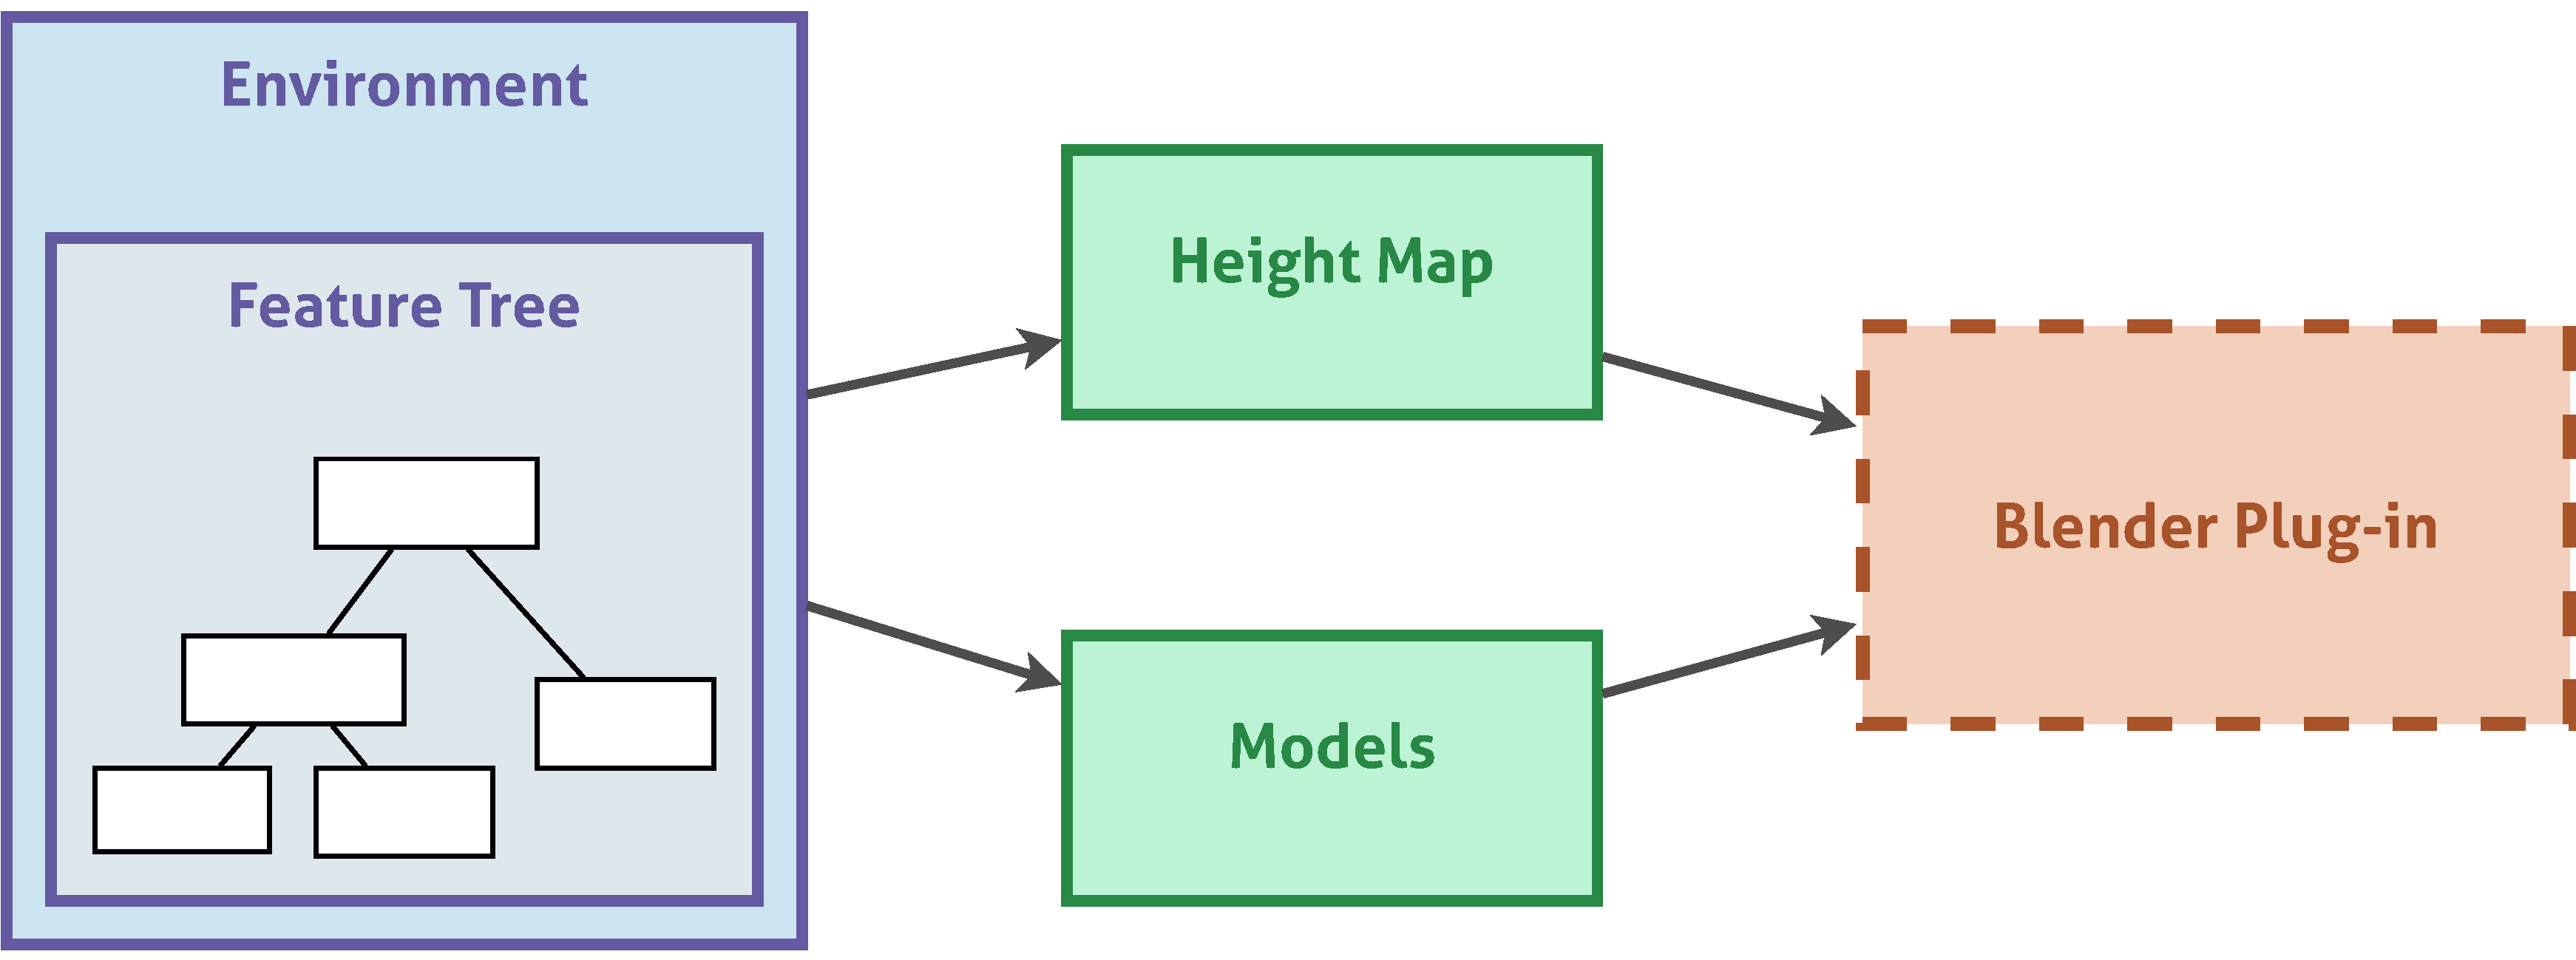
\includegraphics[width=10cm]{env_global.pdf}
    \end{center}
  \end{figure}
\end{frame}

\begin{frame}{Features}
  \begin{itemize}
    \item Forest
    \item Mountain
    \item Road
    \item Cities
    \item Water (river, lake)
    \item ...
  \end{itemize}
\end{frame}

\begin{frame}{Features}
  \begin{figure}
    \begin{center}
      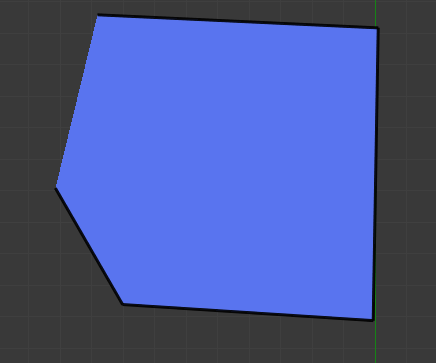
\includegraphics[width=4cm]{feature}
    \end{center}
  \end{figure}
  Feature:
  \begin{itemize}
    \item {\color{Cerulean}shape}
    \item \texttt{z(x,y)} : height function
    \item \texttt{models} : list of models
  \end{itemize}
\end{frame}

\begin{frame}{Tree Construction}
  \only<1>{
  \begin{figure}
    \begin{center}
      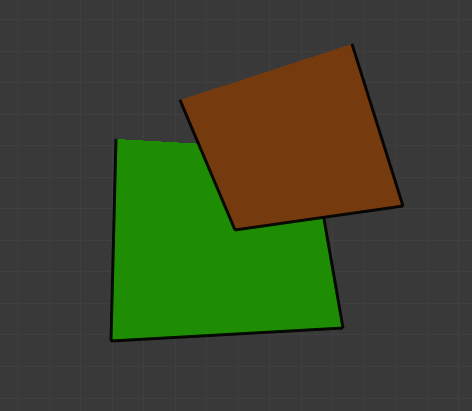
\includegraphics[width=4cm]{feature_2}
    \end{center}
  \end{figure}
  }
  
  \begin{figure}
    \begin{center}
      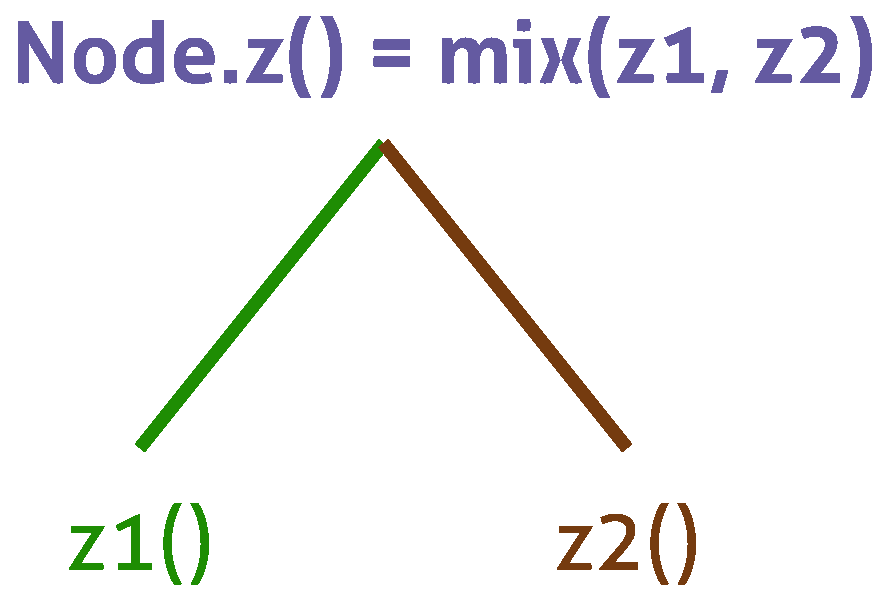
\includegraphics[width=5cm]{mix}
    \end{center}
  \end{figure}
  
  \only<2>{
  Depending on features, \texttt{mix(z1, z2)} could be:
  \begin{description}
    \item[Blend]:  Mean(z1(), z2())
    \item[Addition]: z1() + z2()
    \item[Replace]: Fixed to z1()
  \end{description}
  }
\end{frame}

\begin{frame}{Height Map Generation}
  bla
\end{frame}

\begin{frame}{Demo}
\end{frame}

\begin{frame}{What is missing}
  \begin{itemize}
    \item Live modifications
  \end{itemize}
\end{frame}

\bgroup
\setbeamercolor{background canvas}{bg=black}
\begin{frame}[plain]{}
\end{frame}
\egroup


\begin{frame}{Bibliography}
  
\end{frame}

\begin{frame}{Theme}
  Used the theme \emph{mtheme} by Matthias Vogelgesang, licensed under a Creative Commons
  Attribution-ShareAlike 4.0 International License.
\end{frame}

\end{document}
